
\usetikzlibrary{calc}
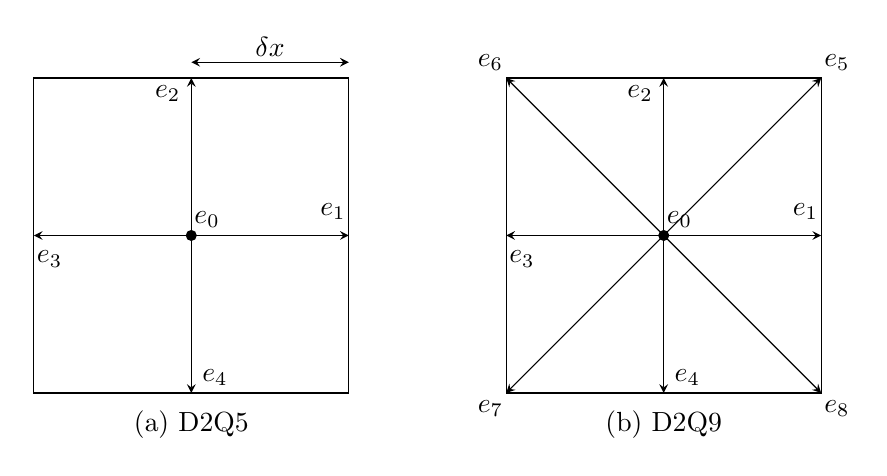
\begin{tikzpicture}[scale=2]
%styledesnœuds
\tikzstyle{textLine}=[rectangle, text=black]
\tikzstyle{textw}=[rectangle, text=black]
\tikzstyle{vector}=[-stealth,thin,rounded corners=4pt]
%figure

\begin{scope}[shift={(0,0)}]
\node[textLine] at (0,-1.2) {(a) D2Q5};

\draw[] (-1,-1) rectangle + (2,2);
% \draw (0,-1) circle[radius=1pt];
\fill (0,0) circle[radius=1pt];
% \draw (0,1) circle[radius=1pt];
% \draw (-1,-1) circle[radius=1pt];
% \draw (-1,0) circle[radius=1pt];
% \draw (-1,1) circle[radius=1pt];
% \draw (1,-1) circle[radius=1pt];
% \draw (1,0) circle[radius=1pt];
% \draw (1,1) circle[radius=1pt];
\coordinate (e0) at (0,0);
\coordinate (e1) at (1,0);
\coordinate (e2) at (0,1);
\coordinate (e3) at (-1,0);
\coordinate (e4) at (0,-1);
%text
\node[textLine] at ($(e0)+(0.1,0.1)$) {$e_0$ };
\node[textLine] at ($(e1)+(-0.1,0.15)$) {$e_1$ };
\node[textLine] at ($(e2)+(-0.15,-0.1)$) {$e_2$ };
\node[textLine] at ($(e3)+(0.1,-0.15)$) {$e_3$ };
\node[textLine] at ($(e4)+(0.15,0.1)$) {$e_4$ };



\draw[vector] (e0) -- (e1);
\draw[vector] (e0) -- (e2);
\draw[vector] (e0) -- (e3);
\draw[vector] (e0) -- (e4);

\draw[stealth-stealth] ($(e2)+(0,0.1)$) -- ($(e1)+(e2)+(0,0.1)$);
\node[textLine] at  ($(0,0.1)+($(e2)+(0,0.1)$)!0.5!($(e1)+(e2)+(0,0.1)$)$)   {$\delta x$};

\end{scope}



\begin{scope}[shift={(3,0)}]
\node[textLine] at (0,-1.2) {(b) D2Q9};

\draw[] (-1,-1) rectangle + (2,2);
% \draw (0,-1) circle[radius=1pt];
\fill (0,0) circle[radius=1pt];
% \draw (0,1) circle[radius=1pt];
% \draw (-1,-1) circle[radius=1pt];
% \draw (-1,0) circle[radius=1pt];
% \draw (-1,1) circle[radius=1pt];
% \draw (1,-1) circle[radius=1pt];
% \draw (1,0) circle[radius=1pt];
% \draw (1,1) circle[radius=1pt];
\coordinate (e0) at (0,0);
\coordinate (e1) at (1,0);
\coordinate (e2) at (0,1);
\coordinate (e3) at (-1,0);
\coordinate (e4) at (0,-1);

\coordinate (e5) at (1,1);
\coordinate (e6) at (-1,1);
\coordinate (e7) at (-1,-1);
\coordinate (e8) at (1,-1);
%text
\node[textLine] at ($(e0)+(0.1,0.1)$) {$e_0$ };
\node[textLine] at ($(e1)+(-0.1,0.15)$) {$e_1$ };
\node[textLine] at ($(e2)+(-0.15,-0.1)$) {$e_2$ };
\node[textLine] at ($(e3)+(0.1,-0.15)$) {$e_3$ };
\node[textLine] at ($(e4)+(0.15,0.1)$) {$e_4$ };

\node[textLine] at ($1.1*(e5)$) {$e_5$ };
\node[textLine] at ($1.1*(e6)$) {$e_6$ };
\node[textLine] at ($1.1*(e7)$) {$e_7$ };
\node[textLine] at ($1.1*(e8)$) {$e_8$ };

%vecteur

\draw[vector] (e0) -- (e1);
\draw[vector] (e0) -- (e2);
\draw[vector] (e0) -- (e3);
\draw[vector] (e0) -- (e4);
\draw[vector] (e0) -- (e5);
\draw[vector] (e0) -- (e6);
\draw[vector] (e0) -- (e7);
\draw[vector] (e0) -- (e8);


\end{scope}
\end{tikzpicture}
